\documentclass[anon,12pt]{colt2022} % Anonymized submission
%\documentclass[final,12pt]{colt2022} % Include author names

% The following packages will be automatically loaded:
% amsmath, amssymb, natbib, graphicx, url, algorithm2e

\usepackage{amsfonts}

\def\R{{\mathbb{R}}}
\def\pr{{\textrm Pr}}
\def\E{{\mathbb E}}
\def\X{{\mathcal X}}
\def\Y{{\mathcal Y}}
\def\H{{\mathcal H}}
\def\G{{\mathcal G}}
\def\B{{\mathcal B}}
\def\yh{{\widehat{y}}}
\def\bias{{\rm bias}}
\def\supp{{\rm supp}}
\def\sign{{\rm sign}}
\def\PL{{\mbox{\rm PL}}}
\newcommand{\predict}{\mathbf{Predict}}
\newcommand{\learn}{\mathbf{Learn}}
\newcommand{\D}{{\cal D}}

\newcommand\bigsubset[1][1.19]{%
   \mathrel{\vcenter{\hbox{\scalebox{#1}{$\subset$}}}}}

\newcommand{\comment}[3]{{\color{#1} {\bf #2 :} #3}}
%\newcommand{\comment}[3]{}  % suppress comments
\newcommand{\sanjoy}[1]{\comment{red}{Sanjoy}{#1}}
\newcommand{\yoav}[1]{\comment{blue}{Yoav}{#1}}

\DeclareMathOperator*{\argmax}{arg\,max}

\title[Active learning using region-based sampling]{Active learning using region-based sampling}
\usepackage{times}
% Use \Name{Author Name} to specify the name.
% If the surname contains spaces, enclose the surname
% in braces, e.g. \Name{John {Smith Jones}} similarly
% if the name has a "von" part, e.g \Name{Jane {de Winter}}.
% If the first letter in the forenames is a diacritic
% enclose the diacritic in braces, e.g. \Name{{\'E}louise Smith}

% Two authors with the same address
\coltauthor{\Name{Sanjoy Dasgupta} \Email{dasgupta@eng.ucsd.edu}\and
\Name{Yoav Freund} \Email{yfreund@eng.ucsd.edu}\\
\addr UC San Diego}

% Three or more authors with the same address:
% \coltauthor{\Name{Author Name1} \Email{an1@sample.com}\\
%  \Name{Author Name2} \Email{an2@sample.com}\\
%  \Name{Author Name3} \Email{an3@sample.com}\\
%  \addr Address}

% Authors with different addresses:
%\coltauthor{%
% \Name{Author Name1} \Email{xyz@sample.com}\\
% \addr Address 1
% \AND
% \Name{Author Name2} \Email{xyz@sample.com}\\
% \addr Address 2%
%}

\begin{document}

\maketitle

\begin{abstract}%
Abstract goes here.
\end{abstract}

\begin{keywords}%
List of keywords
\end{keywords}

\section{Introduction}



\section{Setup}

We assume that examples are drawn from a fixed but unknown
distribution $\D$ over $\X \times \Y$, where $\X$ is a metric space and
$\Y = \{-1,+1\}$~\footnote{In a later section we define the notion of
  neighborhoods more generally to allow, for example, diadic
  partitions}
Given $x \in \X$, the label $y \in \Y$ is drawn
according to the conditional probability function
$$ \eta(x) = \E[Y | X=x] = \pr(Y=1|X=x) - \pr(Y=-1|X=x).$$
The \emph{Bayes-optimal classifier} on $\X$ is $g^*(x) = \sign(\eta(x))$.

The task we wish to solve is \emph{finite population annotation}. We
are given a finite dataset $X \subset \X$ of $n$ points.
We are given the ability to query the label of any point $x \in X$. The
answer to the query: $a(x) \in \{-1,+1\}$ is a binary random variable
drawn according to $\eta(x)$. In particular, multiple queries on the
same point can recieve different answers.

Our goal is to design an active learning algorithm that converges to the Bayes
optimal $g^*(x)$ and does so with a much smaller number of queries
than a passive algorithm.  





We want a procedure that chooses the next point to query. It will be applied repeatedly and then stopped at an arbitrary time, whereupon labels $y(x)$ must be provided for all $x \in X$, including those that were queried. We would like the inferred labels $y(x)$ to approach the Bayes-optimal labels $g^*(x)$ as quickly as possible, ideally much faster than would occur if the query points were chosen uniformly at random.

Specifically, we will be judged on the number of errors on points $x \in X$ with $|\eta(x)| > \gamma$:
$$ \sum_{x \in X} {\bf 1}(y(x) \neq g^*(x),\, |\eta(x)| > \gamma) .$$
The procedure is allowed to fail with probability $\delta$, to account for sampling error.


\section{Active learning algorithm}

\subsection{Sampling regions}

The sampling is organized around a collection $\B$ of measurable subsets of $\X$. These are the atomic sets on which we assess label bias and we call them ``balls''.

\begin{enumerate}

\item[(a)] \emph{Points within a ball.} For any $B \in \B$, let $X_B$ denote the points in $X$ that can be used to assess the bias of $B$. This is simply $X_B = X \cap B$ if $\B$ is a predefined set of balls. 
  
\item[(b)] \emph{Levels of sampling.} We group balls by the number of points that they contain: we put $B$ at {\it level} $\ell$ if
$$ \frac{n}{2^{\ell + 1}} \leq |X_B| < \frac{n}{2^\ell} .$$
Here $\ell$ ranges from $0$ (consisting of balls that contain at least half the data points) to roughly $\lg n$ (containing a single point). 

Let $\B_\ell$ consist of all balls in $\B$ that are at level $\ell$. Thus $\B_0, \B_1, \ldots$ is a partition of $\B$, with $\B_0$ consisting of very large balls and $\B_1, \B_2, \ldots$ consisting of successively smaller balls.

\item[(c)] \emph{The neighborhood of a point.} For any
  $x \in \X$, and level $\ell$.
  $N(\ell,x)$ is the collection of balls from $\B_\ell$ that
  contain $x$.
\item[(d)] We say that the neighborhood $N(x,\ell)$ is {\em covered}
  if there are $k$ query points in each $B \in N(x,\ell)$.
  
\end{enumerate}

\subsection{Bias estimates and provisional labels}

The active learning algorithm uses label-queries to assess the bias of balls $B \in \B$. In turn, these are used to estimate the labels of individual points. All these estimates are organized by sampling level.

\begin{enumerate}

\item[(a)] We take the \emph{bias of a ball} $B \in \B$ to be
$\eta_X(B) = \mbox{average}\{\eta(x): x \in X_B \}$.
At any given time, the algorithm assigns $B$ a qualitative bias estimate,
$$ \yh(B) = 
\left\{
\begin{array}{cl}
+1 & \mbox{significant $+$ bias} \\
-1 & \mbox{significant $-$ bias} \\
0 & \mbox{no significant bias} \\
\bot & \mbox{not yet available}
\end{array}
\right.
$$
The option $\bot$ is used until sufficiently many points in $X_B$ have been labeled: the required number, $k$, is roughly $1/\gamma^2$ (recall that $\gamma$ is the smallest bias that needs to be detected). Once $k$ labels are available, $\yh(B)$ is set to a value in $\{-1,0,+1\}$ and remains fixed thereafter. It will satisfy a basic correctness guarantee (Definition~\ref{def:accurate-bias-estimate}) based on large deviation theory. 

\item[(b)] \emph{Possible labels for a point.} Pick any $x$ and any level $\ell$. Once bias-estimates are available for all balls $B \in \B_\ell(x)$, the possible labels for $x$ at level $\ell$, denoted $\PL_\ell(x) \subset \{-1,0,+1\}$, are defined as follows:
\begin{gather}
+1 \in \PL_\ell(x) \Longleftrightarrow \mbox{there exists $B \in
  \B_\ell(x)$ with $\yh(B) = +1$} \notag \\
0 \in \PL_\ell(x) \Longleftrightarrow \mbox{there exists $B \in \B_\ell(x)$ with $\yh(B) = 0$} \notag \\
-1 \in \PL_\ell(x) \Longleftrightarrow \mbox{there exists $B \in \B_\ell(x)$ with $\yh(B) = -1$}
\label{eq:PL}
\end{gather}
The label of point $x$ at level $\ell$ is a value $\yh_\ell(x) \in \{-1,+1,0,!,\bot\}$. It is initially $\bot$, but once bias-estimates are available for all $B \in \B_\ell(x)$, it is set to a value in $\{-1,+1,0,!\}$ and remains fixed thereafter:
\begin{equation}
\yh_\ell(x) = 
\left\{
  \begin{array}{cl}
+1   & \mbox{if $+1 \in \PL_\ell(x)$ and $-1 \notin PL_\ell(x)$} \\
-1   & \mbox{if $+1 \notin \PL_\ell(x)$ and $-1 \in PL_\ell(x)$} \\
!    & \mbox{if $+1 \in \PL_\ell(x)$ and $-1 \in PL_\ell(x)$} \\
0    & \mbox{if $\PL_\ell(x)=\{0\}$} \\
\bot & \mbox{if $\PL_\ell(x)=\emptyset$}
\end{array}
\right.
\label{eq:provisional-label}
\end{equation}
A point $x$ for which $\yh_\ell(x)=!$ is said to have a ``conflict at
level $\ell$''.

\end{enumerate}

\subsection{The algorithm}

\begin{figure}[h!]
\framebox{
\begin{minipage}[t]{5.9in}
\begin{itemize}
\item{\bf Initialize:} set $\ell=0$, cover all of the balls in $\B_0$.
\item   $\predict(x)$
  \begin{itemize}
  \item Predict with $\yh_\ell(x)$
  \end{itemize}
  \item
  $\learn$  Increment sampling level\\
  Repeat while there is an $x$ that has a conflict at level $0\leq i
  \leq \ell$ and $N(x,i+1)$ is not fully covered. 
  \begin{itemize}
  \item Cover $N(x,i+1)$ using $m$ queries
  \item Query $m$ points uniformly from the domain (background
    sampling)
  \item Update $\yh_{i+1}(y)$ For all $y$.
  \end{itemize}
  Let $\ell+1 \to \ell$
\end{itemize}
\end{minipage}}
\caption{The active learning algorithm. In each iteration, (at most) one focused query and one background query are made.}
\label{alg:main}
\end{figure}


\begin{figure}[h!]
\framebox{
\begin{minipage}[t]{5.9in}
\begin{itemize}
\item Initialize uncertainty regions at all levels:
\begin{itemize}
\item $U_0 = X$
\item $U_\ell = \emptyset$ for $\ell \geq 1$
\end{itemize}
\item Initialize all neighborhoods to ``not yet sampled'':
\begin{itemize}
\item For all $B \in \B$: \ $\yh(B) = \bot$
\end{itemize}
\item Initialize all point-labels, at all levels, to ``not yet available'':
\begin{itemize}
\item For all $x \in X$ and $\ell \geq 0$: \ $\yh_\ell(x) = \bot$
\end{itemize}
%
%\vspace{.1in}
\item Repeat (main loop):
\begin{itemize}
\item If there is a level $\ell \geq 0$ such that $U_\ell \neq \emptyset$:
\begin{itemize}
\item Let $\ell$ be the smallest such level
\item Set query region:
$$ S =  \bigcup_{x \in U_\ell} \bigcup_{B \in \B_\ell(x)} X_B $$
\item {\tt Query}($S$) \ (this queries one point from $S$)
\end{itemize}
\item Background sampling: {\tt Query}($X$)
\item For any neighborhood $B$ that is now adequately sampled for the first time: 
\begin{itemize}
\item Compute bias estimate $\yh(B) \in \{-1,0,+1\}$
\end{itemize}
\item For any $\ell \geq 0$ and $x \in X$ for which $\B_\ell(x)$ is available for the first time:
\begin{itemize}
\item Set $\PL_\ell(x)$ and $\yh_{\ell}(x)$ as per equations (\ref{eq:PL}) and (\ref{eq:provisional-label})
\end{itemize}
\item Update uncertainty region at all levels:
\begin{itemize}
\item $U_0 = \{x \in X: \yh_0(x) = \bot\}$
\item For all levels $\ell \geq 1$: $U_\ell = \{x \in X: \yh_{\ell-1}(x) = \,!, \ \yh_\ell(x) = \bot\}$
\end{itemize}
\end{itemize}

\end{itemize}

\end{minipage}}
\caption{The active learning algorithm. In each iteration, (at most) one focused query and one background query are made.}
\label{alg:main}
\end{figure}



\begin{figure}[h!]
\framebox{
\begin{minipage}[t]{5.9in}

\vspace{.1in}
\emph{Initialization:}
\begin{itemize}
\item Set $Q = \emptyset$ (points queried so far)
\item For each $x \in X$: choose $T_x \sim \mbox{unif}[0,1]$
\end{itemize}

\vspace{.2in}
{\bf Query}($S, \ell$):
\begin{itemize}
\item Query all points in $S \setminus Q$ with $T_z \leq 2^\ell k/n$, and add to $Q$
\end{itemize}

\end{minipage}}
\caption{The sampling procedure. Each point $x \in X$ has an associated value $T_x$ chosen uniformly at random from $[0,1]$. This smaller this value, the earlier this point is likely to be queried.} 
\label{alg:sampling}
\end{figure}

The algorithm of Figure~\ref{alg:main} can be run for any amount of time. Whenever it is stopped, the {\it final label} of any $x \in X$ is
\begin{equation}
\yh(x) = 
\left\{
\begin{array}{ll}
\yh_\ell(x) & \mbox{for the largest $\ell < L[x]$ with $\yh_\ell(x) \in \{-1,+1\}$, if such an $\ell$ exists} \\
\mbox{as queried} & \mbox{if there is no such $\ell$ but $x \in Q$} \\
? & \mbox{otherwise}
\end{array}
\right.
\label{eq:final-label}
\end{equation}

\yoav{I don't think there is anything special about a point that has
  been queried, a single query is not enough, we need $k$ queries to
  determine the prediction.}

\section{Analysis of algorithm}

\subsection{Accuracy of bias estimates}

We'll start with a uniform guarantee on the bias estimates for all balls $B \in \B$.

Recall that each point $x \in X$ gets a label $Y \in \{-1,+1\}$ according to the distribution $\eta(x) = \E[Y | X=x]$. For any $B \in \B$ with $X_B \neq \emptyset$, let $\eta_X(B)$ be the average $\eta$-value in $B$, that is,
$$ \eta_X(B) = \frac{1}{|X_B|} \sum_{x \in X_B} \eta(x) .$$
The specific property we need is encapsulated in the following definition.
\begin{definition}
For any $B \in \B$ and $0 < b_1 < b_2$, we say bias estimate $\yh(B) \in \{+1,-1,0\}$ is \emph{$(b_1,b_2)$-accurate} if the following holds:
\begin{itemize}
\item $\yh(B) = +1 \implies \eta_X(B) > b_1$
\item $\yh(B) = -1 \implies \eta_X(B) < -b_1$
\item $\yh(B) = 0 \implies |\eta_X(B)| < b_2$
\end{itemize}
\label{def:accurate-bias-estimate}
\end{definition}

In what follows, take $0 < \delta < 1$ to be a predefined constant, and define
\begin{equation}
c_1 = \sqrt{3 \ln \frac{4|\B|}{\delta}} .
\label{eq:c1}
\end{equation}
\yoav{So $\B$ is defined relative to $X$?}


For any level $\ell$, define threshold $\tau_\ell$ as follows:
\begin{equation}
\tau_\ell = \min \left( \frac{2^{\ell+2}k}{n}, \ 1 \right)
\label{eq:threshold-ell}
\end{equation}
For any $B \in \B_\ell$, define its \emph{query-set} to be $\Gamma(B)
= \{z \in X_B: T_z \leq \tau_\ell\}$. We base our bias-estimate for
$B$ on the labels of points in $\Gamma(B)$. The following is a
consequence of Lemma~\ref{lemma:large-deviation-bounds} in the
appendix.
\yoav{I guess $T_z \leq \tau_\ell$ refers to the poisson sampling
  trick, which is not discussed. I think that initially we should
  define an oracle that provides samples with the desired properties,
  and later we can (in an appendix?) describe how the oracle is implemented.}
\begin{theorem}
Suppose that $k \geq (8c_1/(b_2-b_1))^2$ where $c_1$ is given in (\ref{eq:c1}). 
For each $B \in \B$, let $\widehat{\eta}(B)$ be the average label on the query-set $\Gamma(B)$, and define the bias-estimate $\yh(B)$ as follows:
$$ \yh(B)
= 
\left\{
\begin{array}{ll}
\sign(\widehat{\eta}(B)) & \mbox{if $|\widehat{\eta}(B)| \geq (b_1 + b_2)/2$} \\
0 & \mbox{otherwise}
\end{array}
\right.
$$
With probability $\geq 1-\delta$, all bias estimates $\yh(B)$, for $B \in \B$, are $(b_1,b_2)$-accurate.
\label{thm:accurate-bias-estimates}
\end{theorem}
In what follows, we will assume that this $(1-\delta)$-probability event holds.

\subsection{Mind changes}

As the level of sampling $\ell$ is increased, the label assigned to a data point $x$, which we denote $\yh_\ell(x)$, might also change; it may flip between $+1$ and $-1$ a few times, with stretches of $0$ or $!$ in between.

Recall that $\PL_\ell(x) \subseteq \{-1,+1\}$ denotes the ``possible labels'' for $x$ at level $\ell$. We distinguish two critical levels: $L_0(x)$, a level beyond which the Bayes-optimal label $s = \mbox{sign}(\eta(x))$ is \emph{always} in $\PL_\ell(x)$; and $L_1(x)$, a level beyond which the opposite label, $-s$, is \emph{never} in $\PL_\ell(x)$.

%\begin{figure}
%\begin{center}
%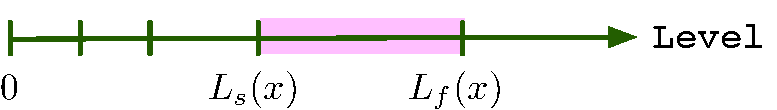
\includegraphics[width=3.5in]{home-stretch.pdf}
%\end{center}
%\caption{The tentative label $\yh_\ell(x)$ of a given point $x$ can undergo several mind-changes as the neighborhood of $x$ is sampled at successively finer levels. Beyond level $L_s(x)$, this $\yh_\ell(x)$ will never be the wrong label, but might be $0$ or $!$. Beyond level $L_f(x)$, the correct label will be assigned.}
%\label{fig:two-levels}
%\end{figure}

\begin{definition}
Pick any $x \in X$ with $\eta(x) \neq 0$ and let $s = \sign(\eta(x))$ be its Bayes-optimal label. We define $L_0(x)$ to be the smallest integer $\ell \geq 0$ such that for all $\ell' \geq \ell$, there exists $B \in \B_{\ell'}(x)$ with $s \cdot \eta_X(B) > b_2$. We define $L_1(x)$ to be the smallest integer $\ell \geq 0$ such that for all $\ell' \geq \ell$, there is no $B \in \B_{\ell'}(x)$ with $s \cdot \eta_X(B) < -b_1$.
\label{defn:L01}
\end{definition}

The key properties of these critical levels are spelled out in the following lemma.
\begin{lemma}
Pick $x \in X$ with $\eta(x) \neq 0$. Let $g^*(x) \in \{+1,-1\}$ be its Bayes-optimal label. Then:
\begin{enumerate}
\item[(a)] For all $\ell \geq L_0(x)$, we must have $g^*(x) \in \PL_\ell(x)$.
\item[(b)] For all $\ell \geq L_1(x)$, we must have $-g^*(x) \not\in \PL_\ell(x)$.
\item[(c)] For all $\ell \geq \max(L_0(x), L_1(x))$, we must have $\yh_\ell(x) = g^*(x)$.
\end{enumerate}
\label{lemma:boundary}
\end{lemma}
\begin{proof}
This lemma follows from the $(b_1, b_2)$-accuracy of the bias estimates for balls. Pick $x \in X$ with $\eta(x) \neq 0$. If $\ell \geq L_0(x)$, there is necessarily a ball $B \in \B_\ell(x)$ with $g^*(x) \eta_X(B) > b_2$ and thus $\yh(B) = g^*(x)$; therefore $g^*(x) \in \PL_\ell(x)$. If $\ell \geq L_1(x)$, every $B \in B_\ell(x)$ has $g^*(x) \eta_X(B) \geq -b_1$ and thus $\yh(B) \in \{0,g^*(x)\}$; therefore $-g^*(x) \not\in \PL_\ell(x)$. Finally, when $\ell \geq \max(L_0(x), L_1(x))$, it follows from (a) and (b) that $\PL_\ell(x) = \{g^*(x)\}$ and thus $\yh_\ell(x) = g^*(x)$.
\end{proof}

\subsection{Bounding the amount of focused sampling}

We can now characterize the points that are queried as part of focused sampling.
\begin{lemma}
For any $\ell \geq 0$, define
\begin{equation}
\Delta_{\ell} \ \ \ = \bigcup_{x \in X: L_1(x) \geq \ell} \bigcup_{B \in \B_{\ell}(x)} X_B .
\label{eq:sampling-region}
\end{equation}
Then, all focused samples at level $\ell$ lie in $\{z \in \Delta_\ell: T_z \leq \tau_\ell \}$.
\label{lemma:focused}
\end{lemma}
\begin{proof}
Let $\overline{U}_\ell$ denote the set of all points that are ever (in any round of sampling) in the uncertainty set at level $\ell$. For any point $x$ with $L_1(x) < \ell$, we have from Lemma~\ref{lemma:boundary}(b) that $\PL_{\ell-1}(x)$ is either $\{\}$ or $\{g^*(x)\}$; either way, $x$ is not in the uncertainty set at level $\ell$. Thus $\overline{U}_\ell \subset \{x \in X: L_1(x) \geq \ell\}$.

The focused samples at level $\ell$ lie in
$$
\bigcup_{x \in \overline{U}_\ell} \bigcup_{B \in \B_\ell(x)} \{z \in X_B: T_z \leq \tau(B) \}
\ \ \ 
\bigsubset[1.44]
\ 
\bigcup_{x \in X: L_1(x) \geq \ell} \bigcup_{B \in \B_\ell(x)} \{z \in X_B: T_z \leq \tau_\ell \} .
$$
This is precisely $\{z \in \Delta_\ell: T_z \leq \tau_\ell \}$.
\end{proof}

A final property we will need for label complexity bounds is that various subsets of interest contain roughly the expected number of points at each level.
\begin{lemma}
Pick any positive integer $\ell_f$. With probability at least $1-2(\ell_f+1)e^{-k/3}$, the following hold for all levels $0 \leq \ell \leq \ell_f$.
\begin{enumerate}
\item[(a)] $|\{x \in X: T_x \leq \tau_\ell\}| \leq 2 n \tau_\ell$.
\item[(b)] If $|\Delta_\ell| \geq k$ then $|\{x \in \Delta_{\ell}: T_x \leq \tau_\ell\}| \leq 2 |\Delta_\ell| \tau_\ell$.
\end{enumerate}
\label{lemma:level-distribution}
\end{lemma}
\begin{proof} 
Pick any subset $S \subset X$ and let $m = |S|$. Then $|\{x \in S: T_x \leq \tau_\ell\}|$ has a $\mbox{binomial}(m, \tau_\ell)$ distribution with expectation $m \tau_\ell$. The probability that it is more than twice its expected value is, by a multiplicative Chernoff bound, at most $e^{-m/3}$.

Both parts follow from this principle; and we take a union bound over all $\ell_o + 1$ levels.
\end{proof}

\subsection{Label complexity bounds} 

\yoav{I think this is the main theorem, however, I find it very hard
  to parse. In particular, I don't see any reference to the fraction
  of examples that are in the focused group at each level. These
  fractions have to be small in order for our sampling to be effective.}

\begin{theorem}
Pick any $0 < \delta < 1$. Suppose that $k \geq (8c_1/(b_2-b_1))^2$, where $c_1$ is defined in (\ref{eq:c1}), and that the active learning algorithm is allowed to make $m$ queries. Let
$$ \ell_0 = \left\lfloor \lg \frac{m}{32k} \right\rfloor $$
and let $\ell_1$ be the largest integer such that
$$ \sum_{\ell = \ell_0 + 1}^{\ell_1} |\Delta_{\ell}| \, \tau_\ell \ \leq \ \frac{m}{8} .$$
Then with probability at least $1-2\delta$, any point $x \in X$ with $L_0(x) \leq \ell_0$ and $L_1(x) \leq \ell_1$ will have final label $\yh(x) = g^*(x)$.
\label{thm:label-complexity}
\end{theorem}
\begin{proof}
Under the setting of $k$, the high-probability events of Theorem~\ref{thm:accurate-bias-estimates} and Lemma~\ref{lemma:level-distribution} hold with probability at least $1-2\delta$. We will henceforth take these for granted.

Denote the first $m/2$ queries by {\it phase one} and the second $m/2$ by {\it phase two}. We will analyze the effect of background sampling in phase one and focused sampling in phase two. We start with the former.

Of the $m/2$ queries in phase one, at least $m/4$ will be background samples. Therefore the $m/4$ points with lowest $T_x$ values are guaranteed to be queried. Now, for $\ell_0$ as defined, we have from (\ref{eq:threshold-ell}) that $\tau_{\ell_0} \leq m/8n$ and from Lemma~\ref{lemma:level-distribution}(a) that at most $m/4$ points in $X$ satisfy
$$ T_x \leq \tau_{\ell_0} \leq \frac{m}{8n}.$$
Therefore all such points are queried in phase one, and thus all balls $B$ at level $\leq \ell_0$ are processed and get bias estimates $\yh(B)$.

It then follows from Lemma~\ref{lemma:boundary} that the following holds for any $x \in X$ with $L_0(x) \leq \ell_0$:
\begin{enumerate}
\item[(a)] For any $\ell \geq \ell_0$, if $\yh_\ell(x)$ is defined then it is either $g^*(x)$ or $!$.
\item[(b)] If $x$ ever leaves $U$ during phase two, then its final label as defined in (\ref{eq:final-label}) is $\yh(x) = g^*(x)$.
\item[(c)] If $x$ is processed at level $L_1(x)$, then it will leave $U$ for good.
\end{enumerate}

Now let's move on to phase two. Let $A = \{x \in X: L_0(x) \leq \ell_0, L_1(x) \leq \ell_1\}$. We will show that every point in $A$ must leave the uncertainty set at some time during phase two. From (b), we can conclude that all these points have their final labels set correctly, once and for all.

We will break the argument into three cases. 

{\it Case 1:} Fewer than $m/4$ focused queries are made in phase two. This can only happen if some round of sampling has an empty uncertainty set, meaning that all of $A$ has left $U$ at that point.

{\it Case 2:} A full $m/4$ focused queries are made in phase two, but at least one of them is at level $\ell_1 + 1$. In that round, $U$ cannot contain any $x \in A$, since by (c) all such points will leave the uncertainty set by level $\ell_1$.

{\it Case 3:} A full $m/4$ focused queries are made in phase two, all at levels $\leq \ell_1$. By the analysis of phase one, none of these queries can be at level $\leq \ell_0$ and by Lemma~\ref{lemma:focused}, the total number of possible focused queries at levels $\ell_0+1$ through $\ell_1$ inclusive is at most
$$\sum_{\ell=\ell_0+1}^{\ell_1} |\{z \in \Delta_{\ell}: T_z \leq \tau_\ell \}| 
\ \leq \ 
\sum_{\ell=\ell_0+1}^{\ell_1} 2 |\Delta_{\ell}| \tau_\ell
\ \leq \ 
\frac{m}{4} ,
$$
where the first inequality is from Lemma~\ref{lemma:level-distribution}(b). Thus by the end of the phase two, every $x \in A$ will have been processed until it leaves $U$.
\end{proof}

\section{Label complexity bounds in various settings}

In order to apply Theorem~\ref{thm:label-complexity}, we need two things:
\begin{itemize}
\item An upper bound on the critical level $L_1(x)$ for each $x \in X$, which in turn (via Lemma~\ref{lemma:focused}) will yield an upper bound on the size of the sampling region $\Delta_\ell$ at each level $\ell$.
\item An upper bound on $L_0(x)$ for points $x$ that we expect to be correctly labeled by the end.
\end{itemize}
We now illustrate how this works out in several canonical settings.


\subsection{One-dimensional data with Massart noise}

Suppose $X$ is an arbitrary set of $n$ points in $\X = [0,1]$ and is labeled according to a conditional probability function $\eta: \X \to [-1,1]$ that satisfies the Massart noise condition:
\begin{itemize}
\item The Bayes-optimal labeling is determined by $p$ disjoint open intervals $I_1 = (\lambda_0, \lambda_1), I_2 = (\lambda_1, \lambda_2), \ldots, I_p = (\lambda_{p-1}, \lambda_p)$, where
$$ 0 = \lambda_0 < \lambda_1 < \lambda_2 < \cdots < \lambda_{p-1} < \lambda_p = 1 .$$
Here $\lambda_1, \ldots, \lambda_{p-1}$ are the \emph{boundary points} between intervals.
\item For each $j$, either $\eta(x) > c$ for all $x \in I_j$ or $\eta(x) < -c$ for all $x \in I_j$. In the first case, we write $s(I_j) = +1$ and in the second case, $s(I_j) = -1$.
\end{itemize}
Here $c > 0$ is some constant. 

We will take $\B$ to be all open intervals of $[0,1]$, and $\B(x)$ to be intervals containing the point $x$. The accuracy parameters $b_1, b_2$ will be set so that $0 \leq b_1 < b_2 \leq c$.
\begin{lemma}
Pick any $x \in I_j$, for $1 \leq j \leq p$.
\begin{enumerate}
\item[(a)] $L_0(x) \leq \left\lceil \lg (n/n_j) - 1 \right\rceil$, where $n_j$ is the number of data points in $I_j$.
\item[(b)] $L_1(x) \leq \left\lceil \lg (n/r(x)) - 1 \right\rceil$, where $r(x)$ is the minimum number of data points between $x$ and a boundary point. 
\end{enumerate}
\label{lemma:critical-one-d-massart}
\end{lemma}
\begin{proof}
For (a), define $n_j = |X \cap I_j|$ and notice that $I_j \in \B_{\ell}(x)$ for $\ell = \lceil (\lg n/n_j) - 1 \rceil$. Moreover, $s(I_j) \cdot \eta_X(I_j) > c \geq b_2$. For levels $\ell' > \ell$, we can make a similar argument using a sub-interval $I \subset I_j$ that lies in $\B_{\ell'}(x)$.

For (b), we define $r(x)$ to be either the number of points in the left-interval $(\lambda_{j-1},x]$ (if $j > 1$) or the right-interval $[x, \lambda_j)$ (if $j < p$), whichever is smaller. For $\ell \geq \lceil (\lg n/r(x)) - 1 \rceil$, any $B \in \B(x)$ will lie entirely within $I_j$ and must therefore have $s(I_j) \cdot \eta_X(B) > 0$.
\end{proof}

Using these bounds on the critical levels, we find that all but an $\epsilon$ fraction of $X$ will be correctly classified after making $m = O(\frac{(p-1)\log n}{c^2} \log \frac{p-1}{\epsilon})$ queries.
\begin{theorem}
In the one-dimensional scenario above, there are absolute constants $C_1, C_2, C_3$ for which the following holds. Pick any $0 < \delta < 1$ and take $k \geq (C_1/c^2) \ln (n/\delta)$. Then with probability at least $1-\delta$, after making $m$ queries, the active learning algorithm will correctly classify all but $n \cdot 2^{-C_2 m/(k(p-1))}$ points in any target interval $I_j$ with $n_j/n \geq C_3 k/m$.
\label{thm:one-d-massart}
\end{theorem}

\begin{proof}
Using Lemma~\ref{lemma:critical-one-d-massart}(b), we see that the sampling region at level $\ell$, as defined in (\ref{eq:sampling-region}), is
\begin{align*}
\Delta_\ell \ \ \ 
&= \bigcup_{x \in X: L_1(x) \geq \ell} \bigcup_{B \in \B_{\ell}(x)} (B \cap X) \\
&\bigsubset[1.44] \bigcup_{x \in X: r(x) \leq n/2^\ell} \bigcup_{B \ni x: |B \cap X| < n/2^\ell} (B \cap X) 
.
\end{align*}
This includes at most $2n/2^{\ell}$ points on either side of each boundary point, so $|\Delta_\ell| \leq 4(p-1)n/2^{\ell}$.

We then set $b_1 = 0$, $b_2 = c$ and apply Theorem~\ref{thm:label-complexity} to conclude that $m$ query points are enough to correctly classify all $x \in X$ with $L_0(x) \leq \ell_0$ and $L_1(x) \leq \ell_1$, for
\begin{align*}
\ell_0
&= 
\lg \frac{m}{32k} \\
\ell_1
&=
\ell_0 + \frac{m}{128 k(p-1)},
\end{align*}
and $k \geq (192/c^2)(2 \ln n + \ln (2/\delta))$; in setting $k$, we have used $|\B| = {n \choose 2}$. The theorem statement follows by invoking Lemma~\ref{lemma:critical-one-d-massart}.
\end{proof}

\subsection{One-dimensional data with monotonic $\eta$}

For our next example, we once again take $X$ to consist of $n$ arbitrarily-placed points in $\X = [0,1]$. This time, however, they are labeled according to a conditional probability function $\eta: \X \to [-1,1]$ that is continuous and strictly increasing. Let $\lambda \in (0,1)$ denote the point at which $\eta(\lambda) = 0$.

As before, $\B$ will consist of all open intervals, and $\B(x)$ be will all intervals containing $x$. Given a threshold $\gamma > 0$ such that we do not need to label points with $|\eta(x)| < \gamma$, we can set accuracy parameters $b_2 = \gamma, b_1 = 0$.

\begin{lemma}
Let $\lambda_L, \lambda_R$ be the points at which $\eta(\lambda_L) = -\gamma$ and $\eta(\lambda_R) = \gamma$.
\begin{enumerate}
\item[(a)] Define $n^- = |[0,\lambda_L) \cap X|$ and $n^+ = |(\lambda_R,1] \cap X|$. Then
$$
L_0(x)
\leq
\left\{
\begin{array}{ll}
\lg \lceil (n/n^+) - 1 \rceil & \mbox{if $x > \lambda_R$} \\
\lg \lceil (n/n^-) -1 \rceil & \mbox{if $x < \lambda_L$}
\end{array}
\right.
$$
\item[(b)] For any $x \in X$, let $r(x)$ be the number of points between $x$ and the boundary point $\lambda$. Then
$L_1(x) \leq \left\lceil \lg (n/r(x)) -1 \right\rceil$.
\end{enumerate}
\label{lemma:critical-one-d-monotonic}
\end{lemma}

\begin{proof}
For (a), take $x > \lambda_R$, for instance. The interval $B = (\lambda,1)$ lies in $\B_\ell(x)$ for $\ell = \lceil \lg (n/n^+) - 1 \rceil$ and has $\eta(B) > b_2$. For higher levels $\ell$, we can take a sub-interval of $(\lambda, 1)$ containing $x$.

For (b), we have $r(x) = |[x,\lambda) \cap X|$ if $x < \lambda$, or $|(\lambda, x] \cap X|$ if $x > \lambda$. For any $\ell \geq \lceil \lg (n/r(x)) - 1 \rceil$, no $B \in \B_\ell(x)$ extends to the other side of the boundary; thus $\eta_X(B) \geq 0$.
\end{proof}

In this setting, we are not required to label points in the interval $[\lambda_L, \lambda_R]$, and thus we don't need $L_0(x)$ values for them. However, we do need to bound $L_1(x)$ for \emph{all} points in order to control the size of the sampling region.

With Lemma~\ref{lemma:critical-one-d-monotonic}, the rest of the argument follows the pattern of the previous one-dimensional case.

\begin{theorem}
There are absolute constants $C_1, C_2, C_3$ for which the following holds. Pick any $0 < \delta < 1$ and take $k \geq (C_1/\lambda^2) \ln (n/\delta)$. Then with probability at least $1-\delta$, after making $m \geq C_2 k \max(n/n^+, n/n^-)$ queries:
\begin{enumerate}
\item[(a)] The active learning algorithm will correctly label all but $n \cdot 2^{-C_3 m/k}$ points in $[0,\lambda_L) \cup (\lambda_R,1]$. 
\item[(b)] If $n_o = \min(|X \cap [\lambda_L,\lambda)|, |X \cap (\lambda,\lambda_R]|) > 0$, then all points in $[0,\lambda_L) \cup (\lambda_R,1]$ will be correctly labeled after $C_3 k \lg (n/n_o)$ queries.
\end{enumerate}
\label{thm:one-d-monotonic}
\end{theorem}

\begin{proof}
From Lemma~\ref{lemma:critical-one-d-monotonic}(b), we have that the sampling region at level $\ell$, as defined in (\ref{eq:sampling-region}), is
\begin{align*}
\Delta_\ell \ \ \ 
&= \bigcup_{x \in X: L_1(x) \geq \ell} \bigcup_{B \in \B_{\ell}(x)} (B \cap X) \\
&\bigsubset[1.44] \bigcup_{x \in X: r(x) \leq n/2^\ell} \bigcup_{B \ni x: |B \cap X| < n/2^\ell} (B \cap X) 
.
\end{align*}
This includes at most $2n/2^{\ell}$ points on either side of the boundary, whereupon $|\Delta_\ell| \leq 4n/2^{\ell}$.

By Theorem~\ref{thm:label-complexity}, making $m$ queries will correctly classify all points with $L_0(x) \leq \ell_0$ and $L_1(x) \leq \ell_1$, for
\begin{align*}
\ell_0
&= 
\lg \frac{m}{32k} \\
\ell_1
&=
\ell_0 + \frac{m}{128 k},
\end{align*}
and $k \geq (192/\lambda^2)(2 \ln n + \ln (2/\delta))$. If $m \geq 32k \cdot \max(n/n^+, n/n^-)$, this includes all points in $[0,\lambda_L) \cup (\lambda_R,1]$ with $r(x) \geq n \cdot 2^{-m/128k}$. 
\end{proof}

\subsection{Two-dimensional data with linear boundary}

\subsection{Higher dimension, with dyadic partitioning}

\subsection{Higher dimension, with smoothness conditions}


% Acknowledgments---Will not appear in anonymized version
\acks{We thank a bunch of people and funding agency.}

\bibliography{yourbibfile}

\vfill

\pagebreak

\appendix

\section{Technicalities}

\subsection{Large deviation bounds for the discrete setting}

\begin{lemma}
Fix a confidence parameter $0 < \delta < 1$ and a positive integer $k \geq 6 \ln (4/\delta)$. 

Let $x_1, \ldots, x_m$ be any collection of points. Suppose that the labels $Y_i \in \{-1,1\}$ of these points are independent, with $\E Y_i = \eta(x_i)$. Define
$$ \eta_o = \frac{1}{m} \left( \eta(x_1) + \cdots + \eta(x_m) \right) .$$
Now consider the following estimator $Z$ of this quantity:
\begin{itemize}
\item Each $x_i$ is chosen with probability $q > 0$, independently. Let $N$ be the number of selected points.
\item If $N > 0$, the labels $Y_i$ of the selected points are obtained, and $Z$ is their average.
\end{itemize}
If $qm \geq k + \sqrt{6k \ln (4/\delta)}$, with probability at least $1-\delta$, 
\begin{enumerate}
\item[(a)] $N \geq k$, and 
\item[(b)] $| Z - \eta_o| \leq \sqrt{(48/k) \ln (4/\delta)}$.
\end{enumerate}
\label{lemma:large-deviation-discrete}
\end{lemma}
\begin{proof}
Let's start with (a). Define $c_1 = \sqrt{3 \ln (4/\delta)}$. We'll take $qm = k + \sqrt{6k \ln (4/\delta)} = k + c_1 \sqrt{2k}$ since this is the worst case. By assumption, $k \geq 2c_1^2$ and thus $qm \leq 2k$.

Now, $N$ has a binomial($m,q$) distribution. By a multiplicative Chernoff bound, for $0 < \epsilon < 1$, we have
\begin{align*}
\pr(N \geq qm(1+\epsilon)) &\leq e^{-qm\epsilon^2/3} \\
\pr(N \leq qm(1-\epsilon)) &\leq e^{-qm\epsilon^2/2}
\end{align*}
Take $\epsilon = c_1/\sqrt{qm}$; by the lower bound on $k$, we have $\epsilon \leq 1/2$. Recalling the choice of $c_1$, we see that with probability at least $1-\delta/2$, we get 
$$(1-\epsilon) qm < N < (1+\epsilon) qm .$$
The lower bound implies $N > qm(1-\epsilon) = qm - c_1\sqrt{qm} = k + c_1 \sqrt{2k} - c_1 \sqrt{qm} \geq k$.

For (b), define $C_1, \ldots, C_m \in \{0,1\}$ as random variables indicating whether the corresponding points were selected; that is, $C_i = {\bf 1}(\mbox{$x_i$ was selected})$. The sum of the obtained labels is then $S = C_1 Y_1 + \cdots + C_m Y_m$. Notice that these $C_iY_i \in \{-1,0,1\}$ are independent with $\E[C_iY_i] = q \eta(x_i)$ and $\E[(C_iY_i)^2] = \E[C_i] = q$. Thus their sum $S$ has expectation
$$ \E [S] = \sum_{i=1}^m \E[C_i Y_i] = \sum_{i=1}^m q \eta(x_i) = qm \eta_o $$
and variance
$$ \mbox{var}(S) = \sum_{i=1}^m \mbox{var}(C_iY_i) \leq qm .$$
We can bound the concentration of $S$ around its expected value using Bernstein's inequality,
$$ \pr(|S - \E[S]| \geq t) \leq 2 \exp \left( - \frac{t^2}{2(\mbox{var}(S) + 2t/3)} \right) .$$
Using $t = \epsilon qm$, we then have that $|S - qm \eta_o| \leq \epsilon qm$ with probability at least $1-\delta/2$.

Combining with the high-probability bound on $N$ above, we get
$$ \frac{qm \eta_o - \epsilon qm}{qm(1+\epsilon)} < \frac{S}{N} < \frac{qm \eta_o + \epsilon qm}{qm(1-\epsilon)},$$
whereupon (recalling $Z = S/N$)
$$ 
\eta_o \left( \frac{1}{1+\epsilon} -1 \right) - \frac{\epsilon}{1+\epsilon} < Z - \eta_o < \eta_o \left( \frac{1}{1-\epsilon} - 1 \right) + \frac{\epsilon}{1-\epsilon} .$$
Since $|\eta_o| \leq 1$,
$$ |Z - \eta_o | \leq \max \left( \frac{2\epsilon}{1+\epsilon}, \frac{2\epsilon}{1-\epsilon} \right)
\leq 
4 \epsilon,$$
as claimed.  
\end{proof}

An immediate consequence is the following large deviation bound. Recall that for any ball $B \in \B_\ell$, its query-set $\Gamma(B)$ is $\{z \in X_B: T_z \leq \tau_\ell\}$, where $\tau_\ell$ is defined in (\ref{eq:threshold-ell}).
\begin{lemma}
Suppose that the constant $c_1$ is set as in (\ref{eq:c1}) and that $k \geq 2c_1^2$. With probability at least $1-\delta$, the following is true for all $B \in \B$ with $|X_B| \geq k$:
\begin{enumerate}
\item[(a)] The query set $\Gamma(B)$ has size at least $k$.
\item[(b)] The average label on $\Gamma(B)$, call it $\widehat{\eta}(B)$, satisfies
$\left| \widehat{\eta}(B) - \eta_X(B) \right| \leq 4c_1/\sqrt{k}$.
\end{enumerate}
\label{lemma:large-deviation-bounds}
\end{lemma}
\begin{proof}
These follow by applying Lemma~\ref{lemma:large-deviation-discrete} to each $B \in \B$ and taking a union bound. 
\end{proof}


\end{document}
